% Companion evidence detail; not additional experimental results.
\documentclass[11pt,a4paper]{article}
\usepackage[T1]{fontenc}
\usepackage[utf8]{inputenc}
\usepackage{lmodern}
\usepackage[margin=2.5cm]{geometry}
\usepackage{microtype}
\usepackage{booktabs,tabularx,array,enumitem,xurl,graphicx,placeins}
\usepackage[numbers,sort&compress]{natbib}
\usepackage{xr-hyper}
\usepackage{fvextra}
\usepackage[colorlinks=true,urlcolor=blue,citecolor=blue,linkcolor=blue]{hyperref}
\externaldocument[M-]{main}
\newcolumntype{Y}{>{\raggedright\arraybackslash}X}
\newcolumntype{L}[1]{>{\raggedright\arraybackslash}p{#1}}
\setlength{\emergencystretch}{2em}
\renewcommand{\arraystretch}{1.15}
\title{Everything but the Software:\\Supplementary Case Evidence and Definitions}
\author{Juan Manuel Servera Bondroit}
\date{Draft of 1 November 2026}
\begin{document}
\maketitle
This companion retains the detailed rival-explanation register,
candidate-mechanism audits and historical measurement definitions.
It adds no experimental results or independent human corroboration.
The five-arm prospective protocol is in the main article and current
researcher kit. The consolidation prompt reproduced here is the
historical v4 prompt, not the amended experiment's approved execution source.
\section{Background}\label{sec:background}

\subsection{Software that only grows}\label{sec:decay}

That software decays when it only accumulates features is one of the oldest
observations in software engineering. Lehman's laws of software evolution hold that a
program in real-world use must keep changing, and that its complexity grows as
it evolves unless work is done to maintain or reduce it~\cite{lehman1980laws};
a later formulation adds that its quality will appear to decline unless it is
rigorously maintained and adapted~\cite{lehman1997metrics}. Parnas called the
result software aging, and blamed in part the changes made by people who do
not understand the original design~\cite{parnas1994aging}. Eick and colleagues
found mixed but, on the whole, persuasive evidence of code decay in fifteen-plus
years of change data from a large telephone-switching
system~\cite{eick2001decay}. Cunningham's technical-debt metaphor framed the
cost of not consolidating as interest paid on every later
change~\cite{cunningham1992wycash}, and Fowler's design stamina hypothesis
holds that without attention to design, adding features eventually becomes
slower than it would have been with it~\cite{fowler2007stamina}. Studies have
since put numbers on the interest: across 39 proprietary code bases,
low-quality files had fifteen times more defects and their issues took
124\% longer to resolve in a CodeScene-associated vendor
study~\cite{tornhill2022codered}; 43 developers self-reported losing about
23\% of their working time to technical debt in a longitudinal
study~\cite{besker2018cripples}. These are different outcomes and populations.

The evidence is not universal. Increasing complexity and declining quality
are among the less strongly supported of Lehman's laws, and some systems have
grown without the predicted decay~\cite{herraiz2013laws}. Several findings
above are observational, and their estimates belong to the studied settings,
not every code base.

The engineering intuition often called \emph{software entropy} is that keeping
a changing system coherent requires counter-work: removing obsolete paths,
restoring boundaries and revisiting assumptions. Software does not deteriorate
simply because time passes, and thermodynamic entropy supplies no measure of
its quality. Here the measurable quantities are losses of required behaviour,
excess structural burden and the effort needed for a later change.

\subsection{What carries from one feature to the next?}\label{sec:inheritance}

Feature accumulation is the addition of capabilities and interactions; churn
is the editing activity that implements, replaces or removes them. Neither
is itself deterioration. A \emph{regression} loses previously working
behaviour that is still required. A never-implemented feature is instead an
acquisition failure. Persistence means that the same fault remains unresolved;
propagation means that a later, distinct fault or failure can be traced to
reuse of the earlier one. \emph{Compounding} is the stronger claim that the
earlier error increases subsequent error risk or change burden.

These distinctions matter because an agent inherits more than a code diff.
The repository supplies implementations, tests, interfaces and deployment
assumptions. Instructions, skills and notes supply an account of how to work
on them. A mistaken rule can become code, then a test expectation or an
instruction, and finally the precedent used for another feature. The stored
record need not be correct to become authoritative in the next session.
Conversely, an inherited implementation can be sound even when it differs
from a human reference. The question is what subsequent work can achieve
from that state.

\begin{figure}[!htbp]
\centering
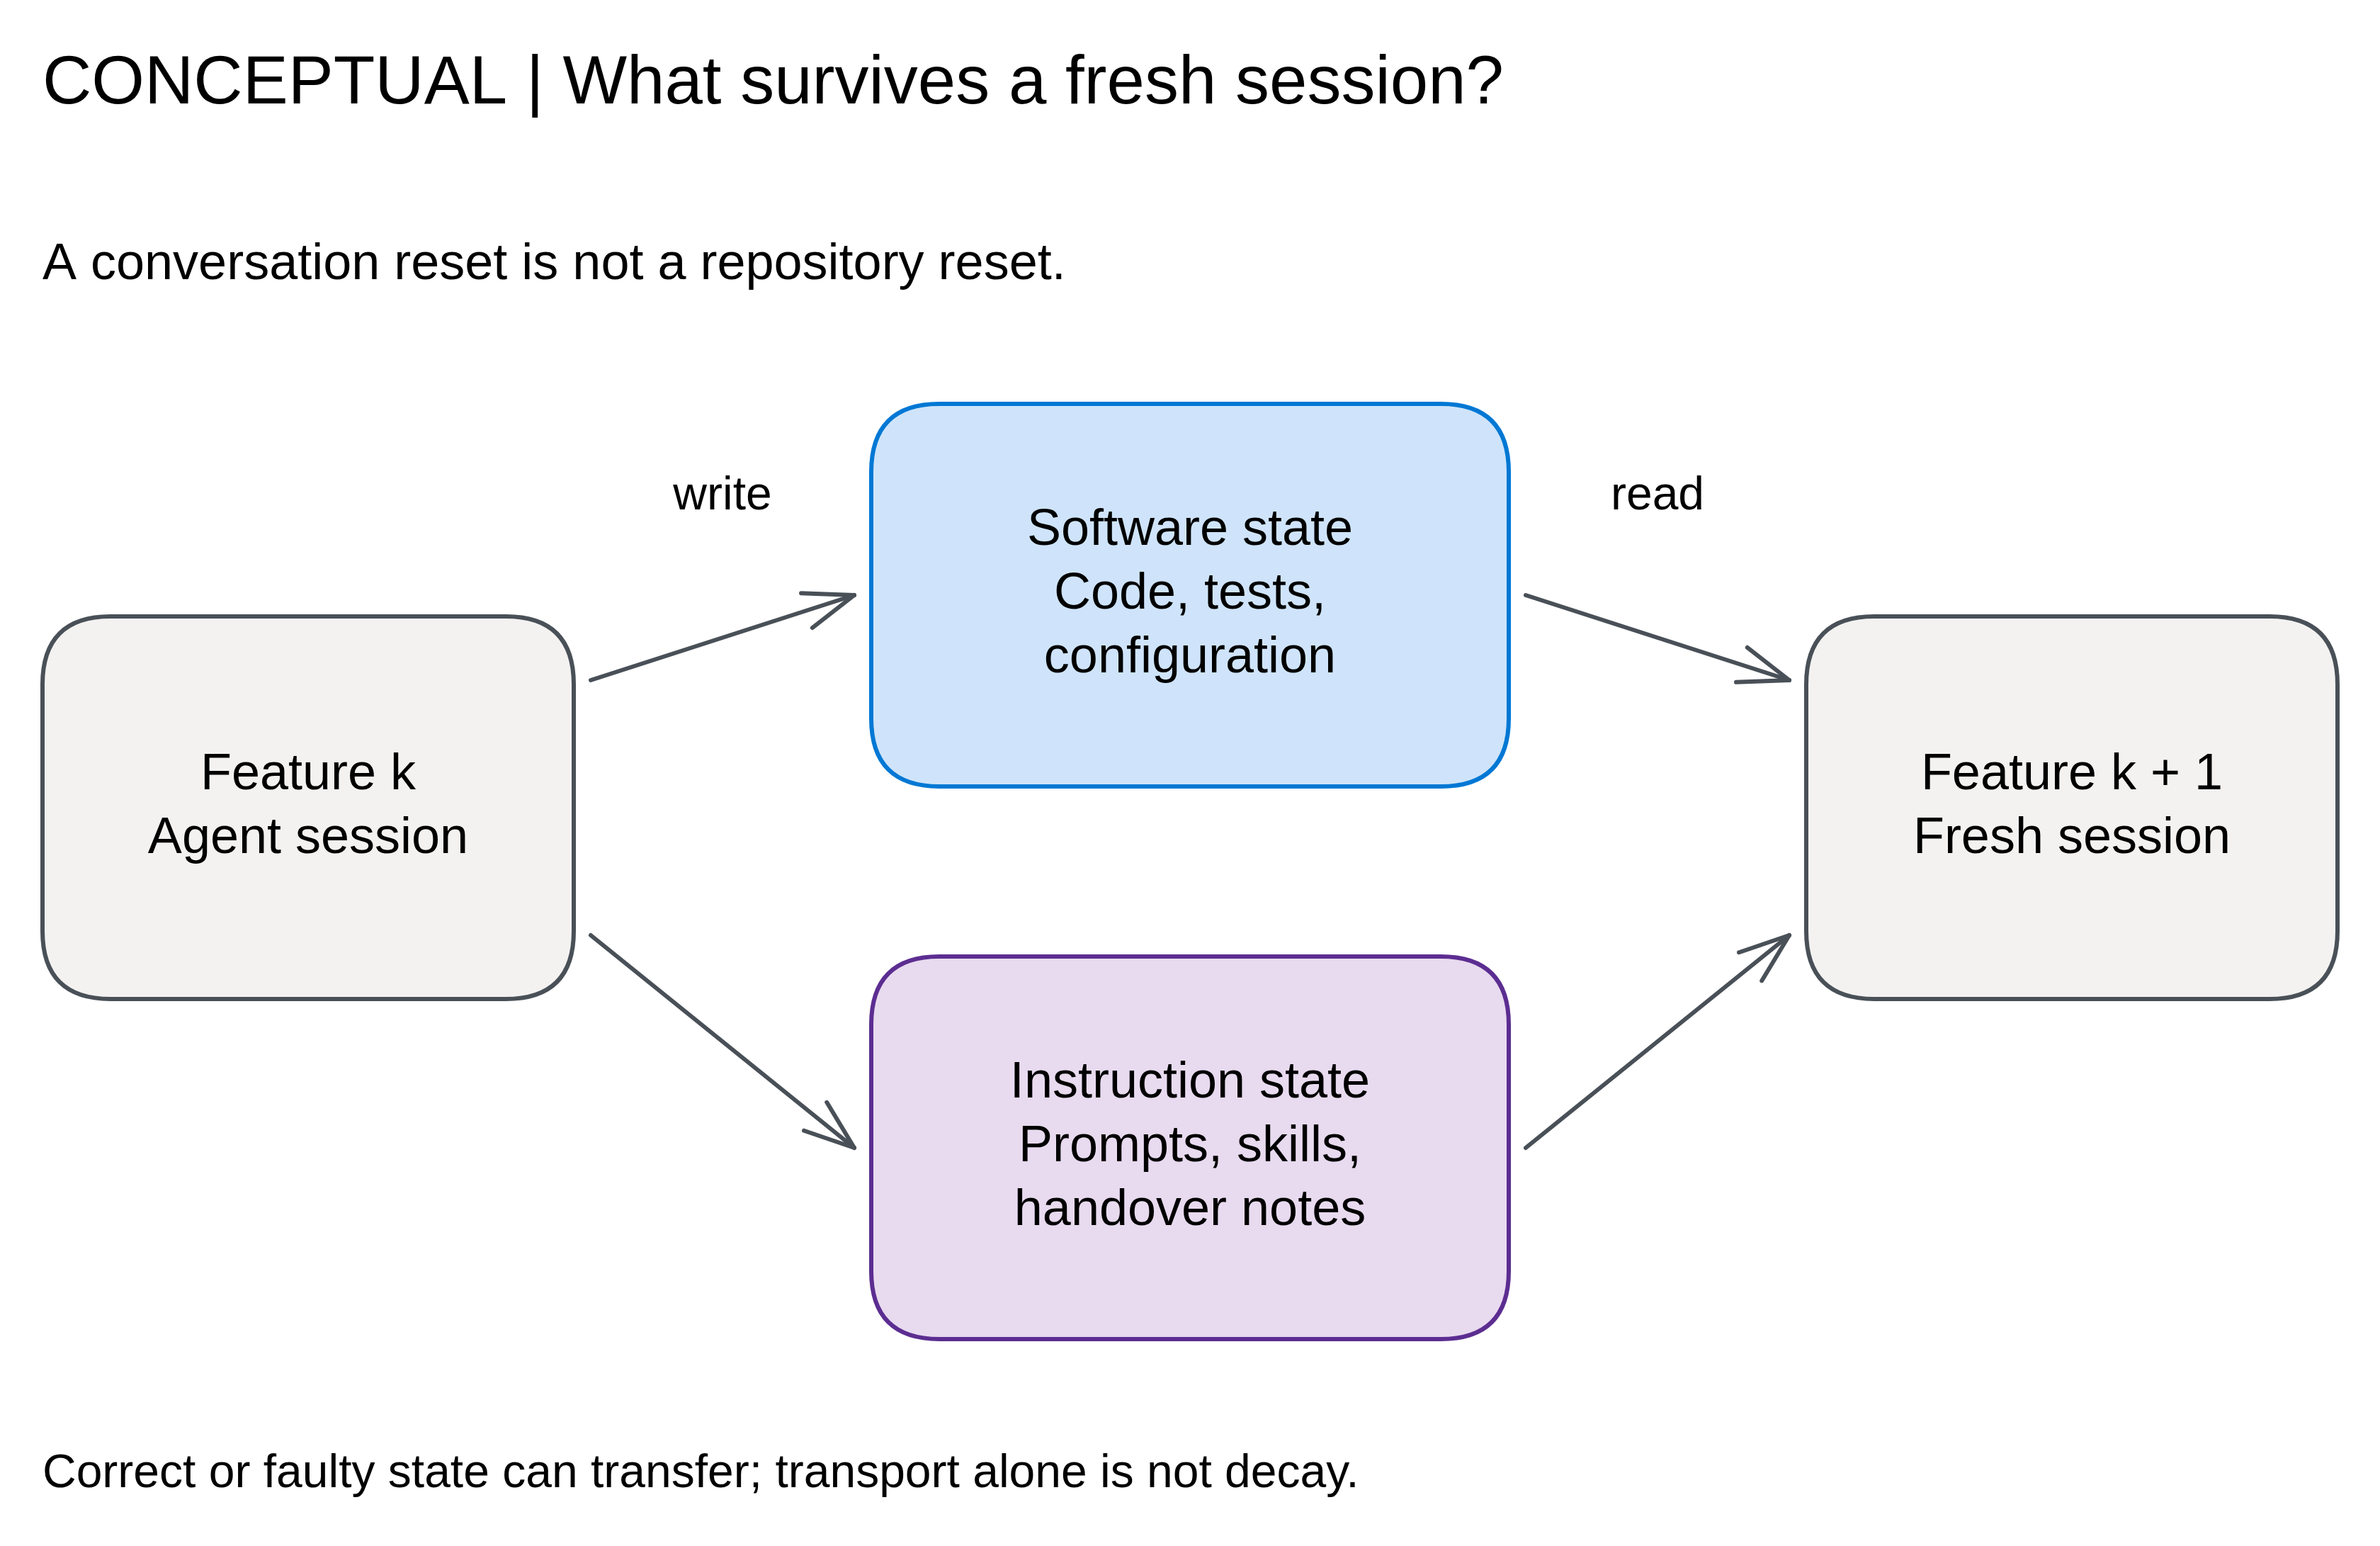
\includegraphics[width=\linewidth]{fig-state-inheritance.png}
\caption{Conceptual state transfer between feature sessions. A fresh
conversation does not reset inherited software or instruction state.
Solid arrows denote possible read/write paths, not measured error
propagation. Both channels can carry correct decisions as well as faults;
their presence alone is not evidence of decay.}\label{fig:stateinheritance}
\end{figure}

Figure~\ref{fig:stateinheritance} separates the two persistent channels from
conversation history. It is an explanatory model, not an observed trajectory
or a claim that every tool retains the same material.

\subsection{Compounding within and between features}\label{sec:empirical}

\paragraph{Errors carried in conversation.}
An earlier answer changes the context from which a model produces the next
one. Experiments on this pathway distinguish dependence on an erroneous
history from the difficulty of a long task.

Zhang et~al.'s earlier \emph{How Language Model Hallucinations Can Snowball}
shows why consistency is not enough. On three question-answering datasets,
ChatGPT and GPT-4 produce false justifications after wrong answers, yet often
reject the individual false claims when questioned in a separate session.
Their explanation is over-commitment to the earlier answer rather than only
a lack of knowledge. The inspected original experiments concern question answering in two
2023 models; the later ICML publication expands the model coverage
~\cite[original preprint, Secs.~3.1--3.4]{zhang2023snowball}.

Sinha et~al. test the distinction directly in a controlled execution task.
Models receive both the lookup dictionary and the plan, then maintain a
running sum. The authors vary the fraction of incorrect answers in artificial
prior histories and measure the accuracy of subsequent state updates, not
merely whether the final total remains correct. More erroneous history reduces
later accuracy beyond the effect of context length. This is counterfactual
evidence of \emph{self-conditioning}: earlier mistakes can increase the chance
of new mistakes. Scaling non-thinking models does not remove the effect, but
Qwen3 models with thinking enabled avoid it in this setup. The result identifies
a dependence on model configuration as well as erroneous history
\cite[Secs.~2.2--3, Figs.~5--6]{sinha2025illusion}.

Laban et~al. supply complementary conversational evidence. Across six
generation tasks, including Python and SQL, they report a 39\% average relative
performance drop when instructions arrive through underspecified multi-turn
conversation rather than all at once. A concatenated-instruction control
largely preserves performance, weakening information loss from rephrasing as
the explanation. Their analyses associate premature answers with lower success
and describe reliance on earlier incorrect attempts and increasingly bloated
solutions. These are simulated conversations and diagnostic analyses, not a
controlled estimate of the cost of a particular inherited coding defect; the
39\% is not a percentage-point loss or a repository defect
rate~\cite[arXiv v1, Secs.~3.3 and~6.1, App.~F.1--F.2]{laban2025lost}.

\paragraph{Errors carried in the repository.}
Pan et~al.'s \emph{SWE-Maintain} preprint tests the pathway most directly
relevant to successive feature work. It reconstructs 100 three-event
maintenance episodes from 50 Python
repositories and runs each later task from two starting points: the developers'
preceding patches and the agent's own preceding changes. Task, agent and tests
are held fixed, and every event uses a fresh session: only the repository
carries the earlier work forward. Across 1,996 paired later events, agent
history lowers new-task resolution by 5.6 percentage points (95\% interval
$[-7.2,-4.1]$). Requiring earlier tests to remain passing widens the gap to
14.0 points. The unweighted mean new-task gap grows from 4.0 points at the second
event to 7.2 at the third, consistent with an accumulating downstream cost,
though three-event episodes cannot establish a general long-horizon decay
law~\cite[Secs.~2.5 and~4.1, Table~2]{pan2026swemaintain}.

Their \texttt{python\_unidiff} example makes the proposed propagation concrete:
an agent splits a string into lines, losing line terminators; the next
task reuses that logic in a constructor, while developer history succeeds.
The framing appears in Figure~1's caption and the detailed failure in
Section~5.1 and Figure~5~\cite{pan2026swemaintain}.
Their \texttt{parse\_crontab} example exposes a less visible dependency:
an agent's local Python~3 fix passes the current and next tests, but later
code relies on module-wide compatibility aliases that it never supplied.
The later compatibility failure is discussed in
Section~5.1 and Figure~5~\cite{pan2026swemaintain}.
Among the 619 later events
whose inherited code passes earlier tests and whose next task is not already
solved, the new-task-only difference is $-1.1$ points (95\% interval
$[-3.8,+1.6]$), and the event-resolution difference is $+2.7$ points (95\% interval
$[-0.5,+6.1]$), with no detected disadvantage. This is a selected clean-history
subset, not a randomised repair intervention, and it does not prove equivalent
maintainability under all changes. It points more directly to inherited
behavioural failures than to structural complexity as the main observed
channel~\cite[Sec.~4.2, Table~3; Sec.~5.1, Fig.~5]{pan2026swemaintain}.

Figure~\ref{fig:inheritedhistory} shows the published event-resolution
contrasts, including the clean-history cohorts. Event resolution requires
the new task and all earlier non-superseded tests to pass. Its larger gap
therefore includes retained failures as well as difficulty solving the new
task. The current-task-only difference of $-5.6$ points is important for the
cross-feature hypothesis precisely because it does not count earlier failing
tests against success on the new task.

\begin{figure}[!htbp]
\centering
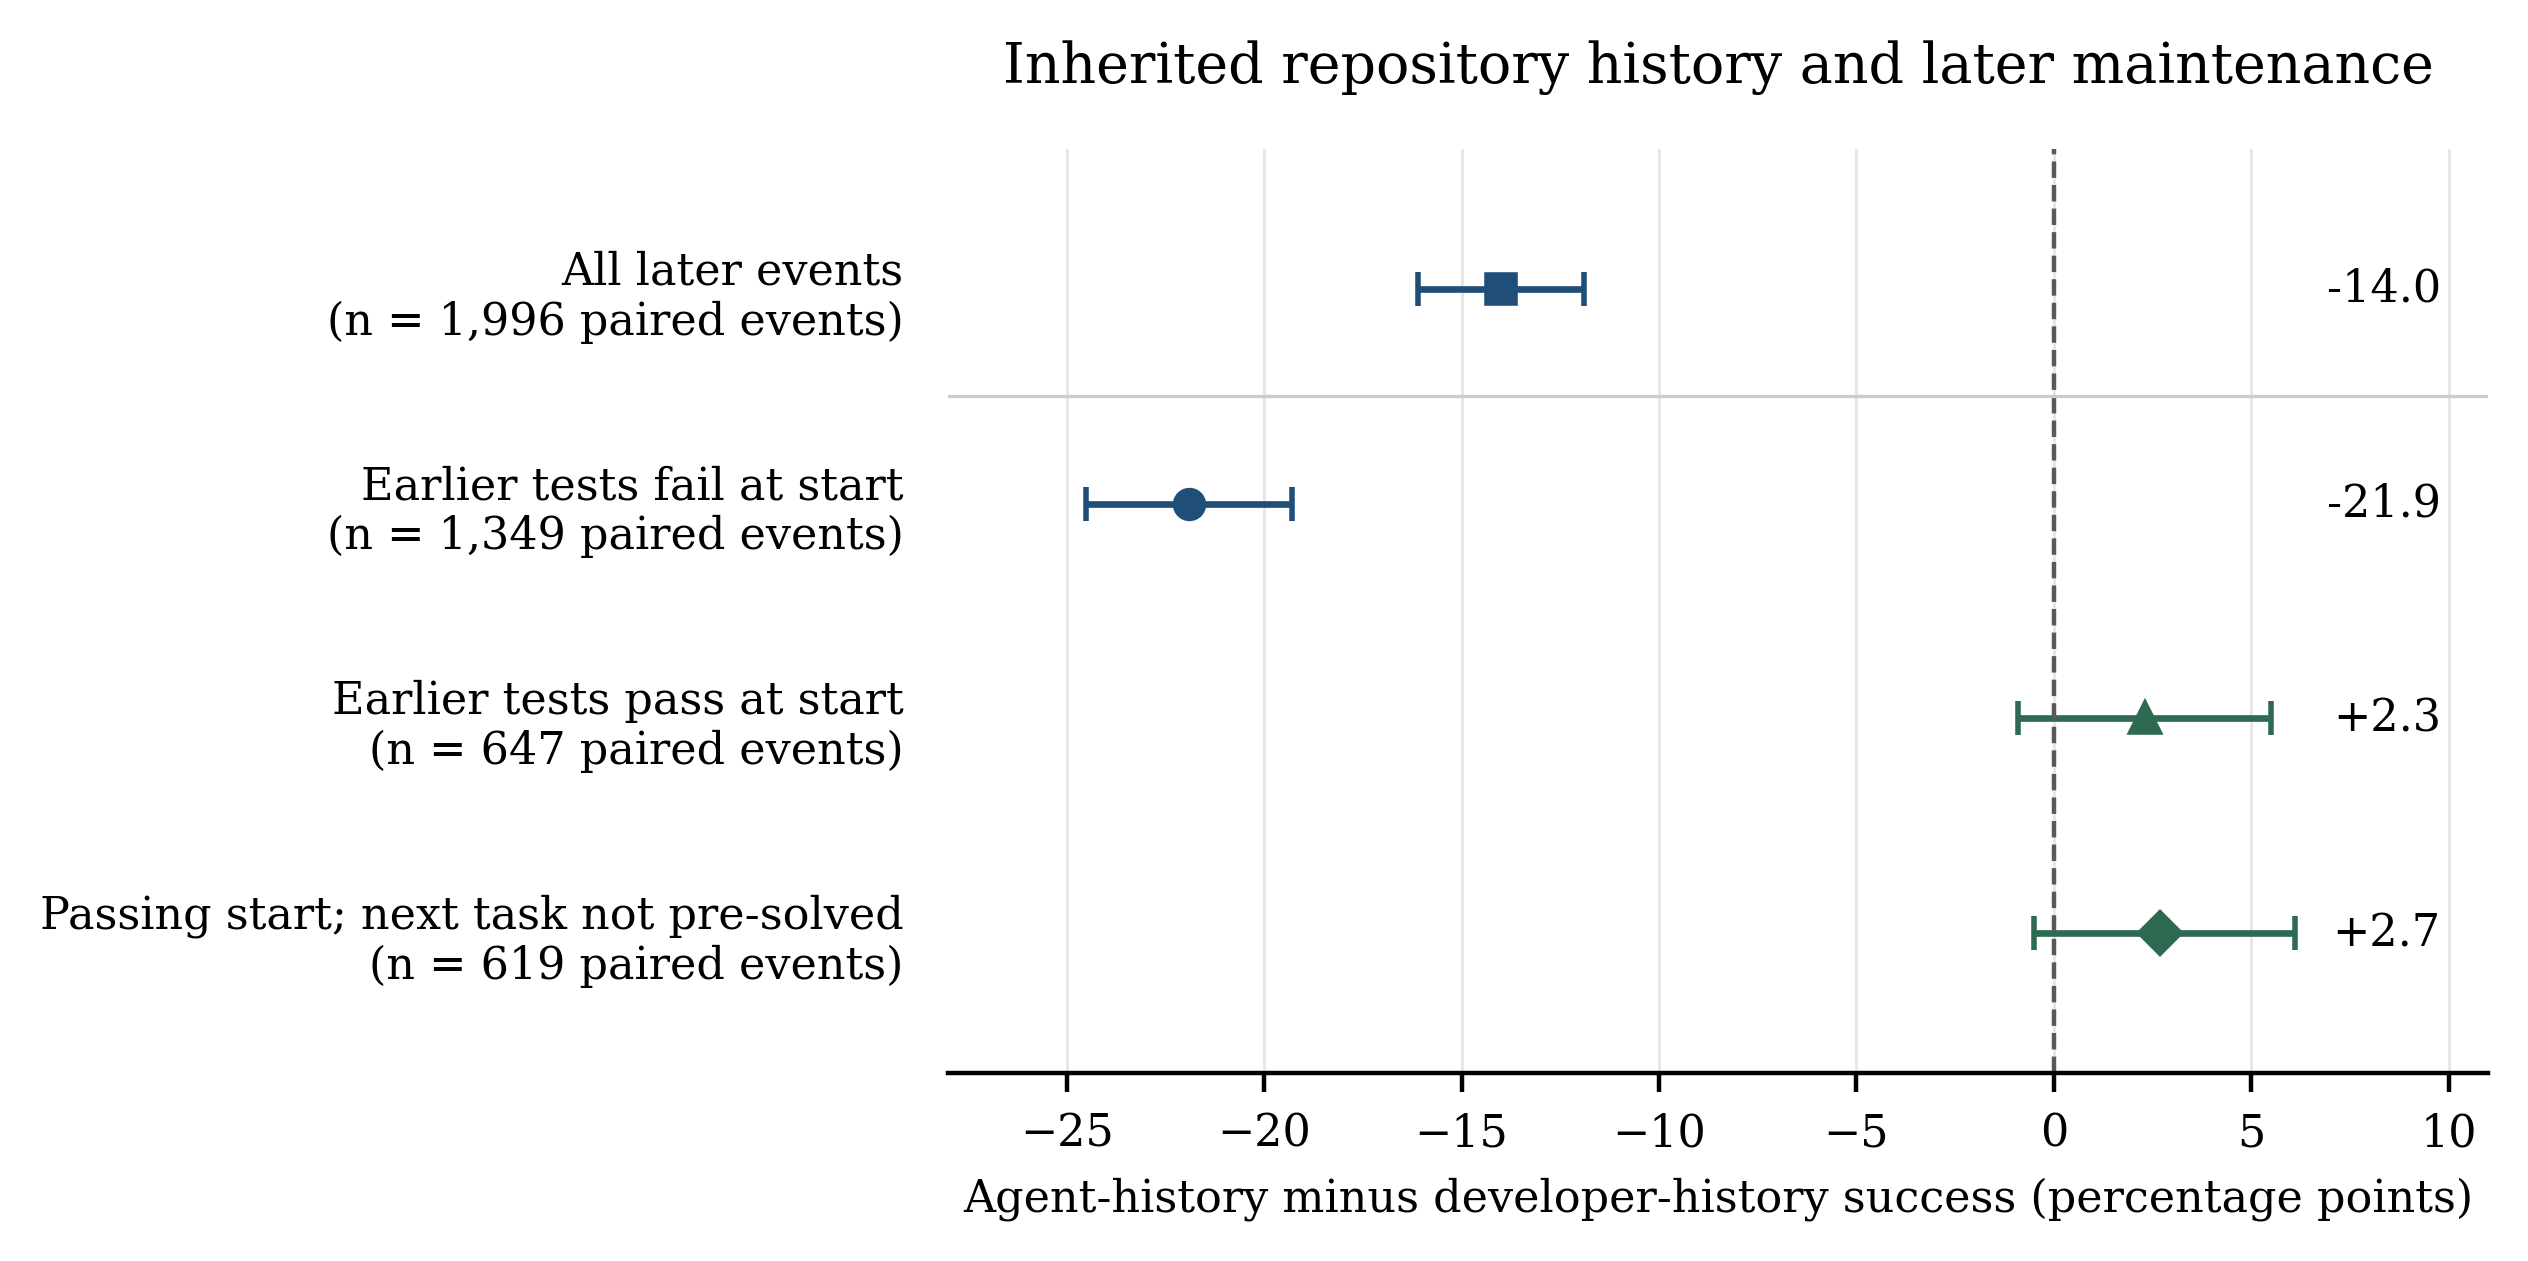
\includegraphics[width=\linewidth]{fig-inherited-history.png}
\caption{Later maintenance from two repository histories. Points and 95\%
repository-clustered bootstrap intervals are transcribed from Pan et~al.,
Table~3~\cite{pan2026swemaintain}. The outcome is event resolution: current
and all earlier non-superseded hidden tests pass. Negative differences favour
developer history. The 1,996 paired events come from 100 three-event episodes
in 50 Python repositories, evaluated with five systems and two models.
Subgroups overlap and are selected by the agent-history starting state;
the last excludes pre-solved and unevaluable tasks. They are not randomised
repair conditions.}\label{fig:inheritedhistory}
\end{figure}

The conversation and repository studies therefore locate two different
transmission pathways. Resetting context addresses the first, but not faulty
code retained for the next feature. SlopCodeBench and SWE-CI extend the
evaluation horizon to iterative structural erosion and behavioural
regressions~\cite{orlanski2026slopcodebench,chen2026sweci}. A maintainability
study using late-2024 coding assistants found no significant downstream
difference; only its second phase was randomised
~\cite{borg2025echoes}. This is assistant-era evidence, not a test of the
current autonomous agents. The emerging
question is which inherited failures survive, how they affect later work,
and which interventions prevent or repair them.

\paragraph{Output and review capacity.}
Understanding changes
is a major challenge of code review; habituation, fragmented context and
uneven retrieval from long contexts may limit scrutiny as output
grows~\cite{bacchelli2013review,yu2026habituation,cemri2025multiagent,liu2024lost,hong2025contextrot}.
Faster feature delivery also shortens the time available to discover that an
earlier assumption has become the foundation of another change. Further
empirical and practitioner context is retained in the ancillary supplement.

\subsection{Corrective instructions as maintenance debt}\label{sec:instructiondebt}

A failed agent action often invites a new instruction: run this check, never
edit that file, remember this exception. GitHub's account of more than
2,500 agent-definition files recommends starting small, testing and adding
detail when an agent makes mistakes~\cite{nigh2025agentsmd}. The resulting
guidance can preserve useful lessons, but it also becomes another maintained
system. Chatlatanagulchai et~al. document ongoing maintenance of this
material~\cite[Secs.~4.2.2--4.2.3]{chatlatanagulchai2026readmes}.
Here \emph{instruction debt} denotes the avoidable burden of obsolete,
duplicated, conflicting or poorly routed directives in prompts, skills and
handover notes. This extends the maintenance question from the product to
the machinery that changes it.

Repository histories show that this material evolves. Mohsenimofidi et~al.
found no post-creation change in 77 of 155 instruction files. In the ten most
frequently changed files, however, they classified 169 commits: 78 added
instructions, 59 modified them and 23 removed them. These are three of nine
categories, with 242 assignments in total, rather than a partition of the
169 commits~\cite[Sec.~4.3, Table~2]{mohsenimofidi2026context}.
Chatlatanagulchai et~al.'s manual analysis of 100 post-adoption commits
produced 78 addition, 32 modification and 19 deletion labels; addition labels
occurred across 66 distinct commits. Figure~\ref{fig:instructionmaintenance}
replots the label counts~\cite[Secs.~4.2.2--4.2.3]{chatlatanagulchai2026readmes}.
These histories contain accumulation and pruning, rather than a uniform
march towards longer files. The authors associate their day-scale edit
intervals with ongoing project maintenance rather than immediate prompt
debugging.

\begin{figure}[!htbp]
\centering
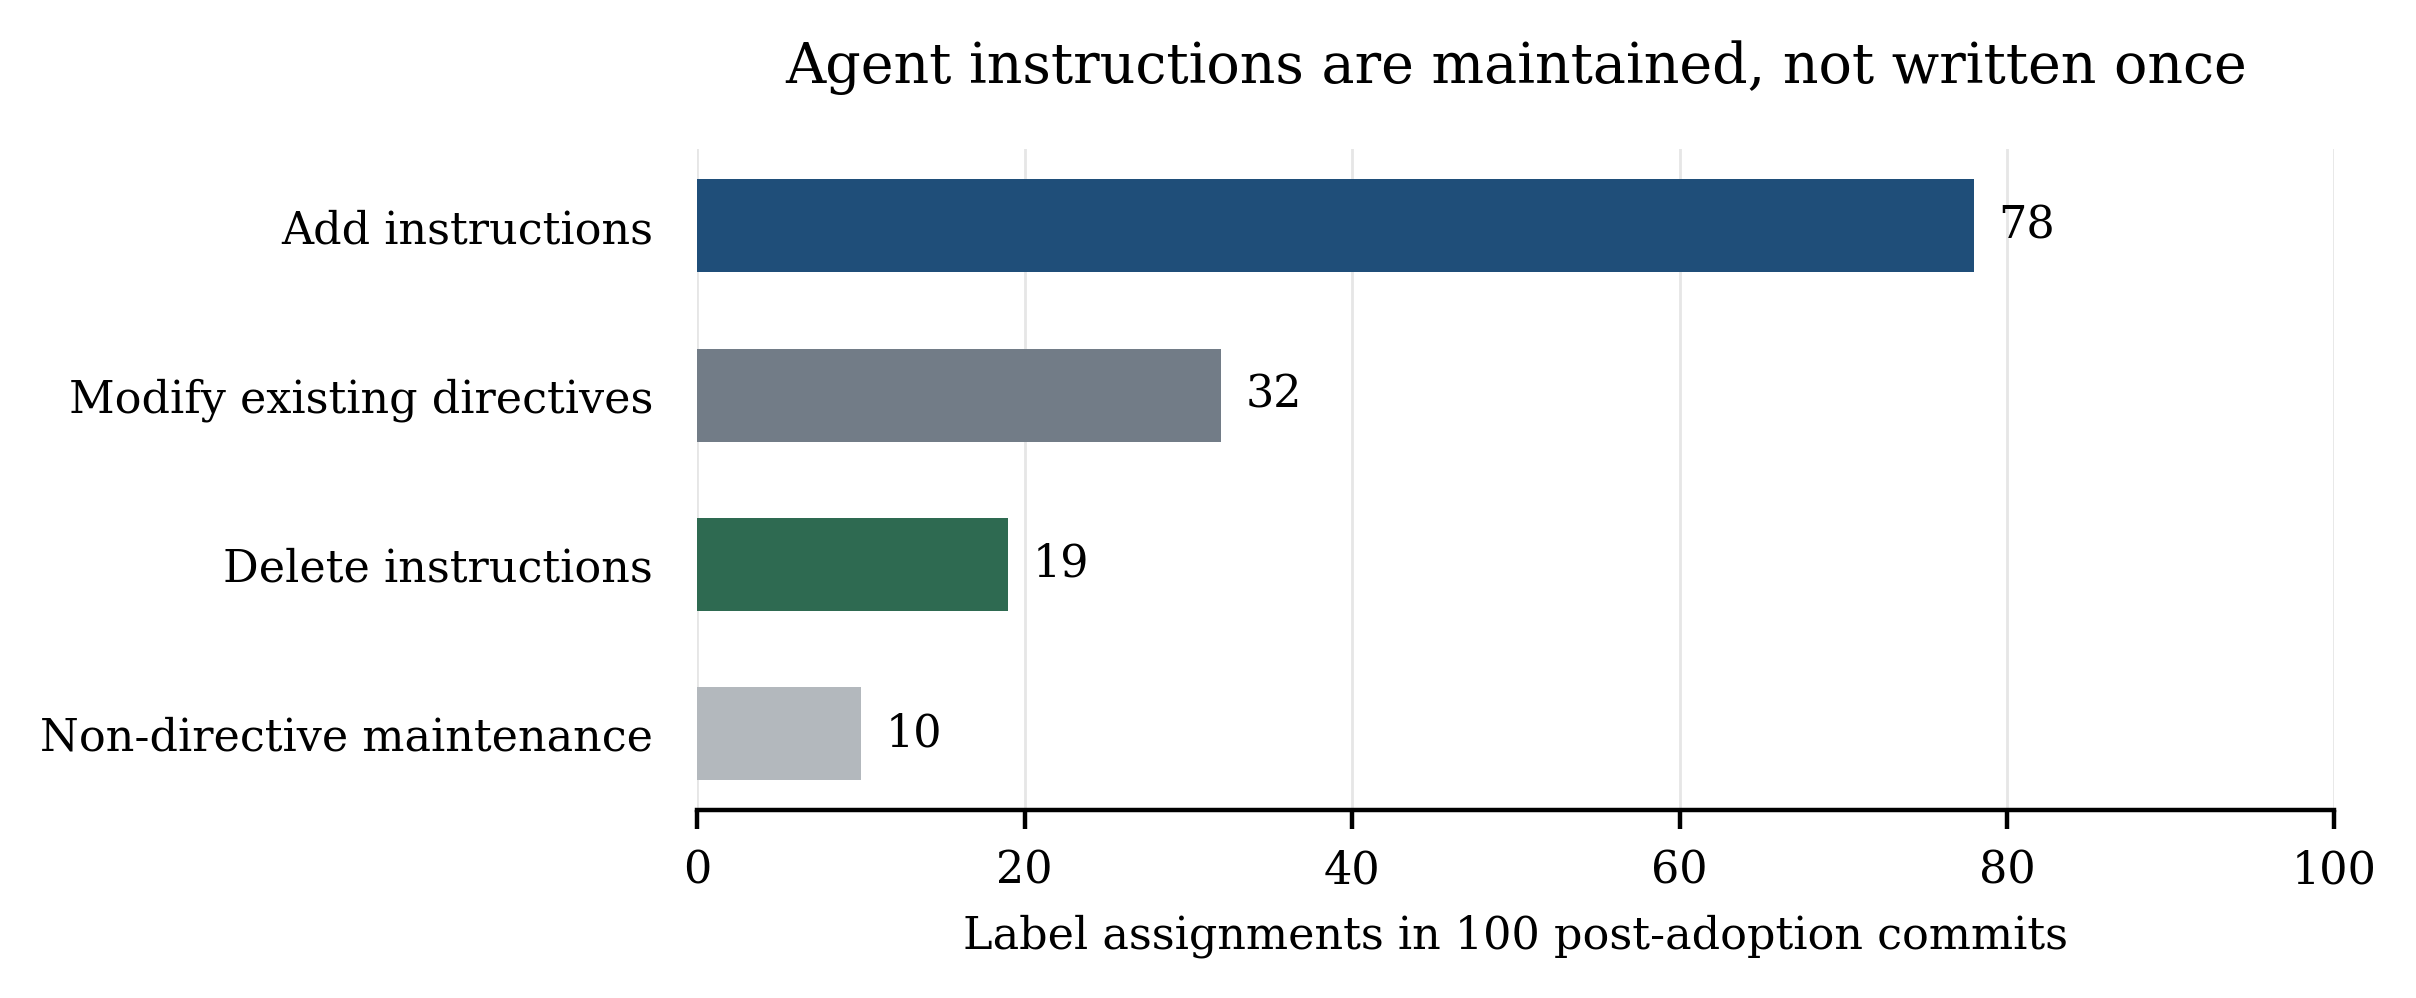
\includegraphics[width=0.94\linewidth]{fig-instruction-maintenance.png}
\caption{Instruction-file maintenance in 100 randomly sampled post-adoption
commits, from Chatlatanagulchai et~al., Sections~4.2.2--4.2.3
\cite{chatlatanagulchai2026readmes}. Commits can receive several labels;
line-level and section-level add/delete labels are combined. The ten
non-directive maintenance labels are the remainder of 139 total assignments.
The chart counts edit types, not net token growth or effects on agent
performance.}\label{fig:instructionmaintenance}
\end{figure}

Gloaguen et~al. test the effect of supplying such context. Across four
agent--model pairings on 300 SWE-bench Lite tasks and 138 CTXbench tasks,
LLM-generated context files increased average inference cost by 20\% and
23\%, respectively; task success was slightly lower, by 0.5 and 2 percentage
points, without significant differences from the no-file baseline.
Developer-written files performed significantly better than LLM-written
files on CTXbench ($p=0.038$). Agents followed the instructions, performed more testing
and exploration, and spent more reasoning tokens. Yet file length did not
explain success, and generated context helped when other documentation was
removed~\cite[Secs.~4.2--4.4, App.~B]{gloaguen2026agentsmd}.
Instruction count and loaded tokens are therefore different exposures from
the obligations and behaviours those instructions induce.

Anthropic's context-engineering account describes the practical tension:
provide enough information to guide action, but avoid brittle prompt logic
and an expanding catalogue of exceptions~\cite{rajasekaran2025context}.
Maintaining these instructions means preserving necessary constraints while
replacing accumulated exceptions with coherent rules, executable checks and
task-specific retrieval. To test the corrective-rule
spiral directly would require versioned instructions, actual session inputs
and outcomes across successive revisions. The testbed record supplies document
growth and rule changes; the consolidation protocol tests a bounded form of
handover maintenance by replacing, rather than appending to, its design note.

SkillOpt supplies counterevidence to treating instruction change as
inherently harmful. Its first-party account describes bounded edits to
skill files, held-out validation and retention of successful versions
without changing the target model's weights~\cite{microsoft2026skillopt}.
Procedural knowledge needs evaluation and maintenance; its length alone
tells us little about its quality.

Jiang et~al.'s preprint compares workflow memory with skills distilled from
the same execution histories. Its paired trajectory analysis associates
skills chiefly with more reliable procedures, while also identifying
misapplication and insufficient runtime verification
\cite[Secs.~3.3, 5.1--5.3]{jiang2026skills}.
This qualifies an instruction-debt account: retained guidance can stabilise
execution rather than merely burden context. Their retrieval study also
separates skill access from task success; in their comparison, lower
exact-match access was observed alongside sustained downstream success
\cite[Sec.~5.5]{jiang2026skills}. Because retrieval diagnostics are run
separately from task execution, this comparison does not isolate the effect
of reduced skill access. Neither result measures the effects of
accumulating repository instructions across feature changes.

\subsection{Refactoring, review and evaluation boundaries}\label{sec:evaluationwork}

Agentic refactoring, review and human correction are already studied.
RefactorBench evaluates 100 handcrafted multi-file refactoring tasks across
nine Python repositories, not scheduled consolidation between feature
additions~\cite{gautam2025refactorbench}. Kumar et~al.'s ASE~2025 study
observed developers collaborating with agents on existing issues: incremental,
active collaboration was associated with greater success, not randomly
assigned to establish an optimal intervention rate~\cite{kumar2025agents}.
SWE-Sharp-Bench supplies a reproducible C\# issue-resolution benchmark and
curation pipeline~\cite{mhatre2025swesharp}; reproducible repository-scale
evaluation itself is not a contribution claimed here.

Two recent preprints sharpen the evaluation problem. CRBugBench evaluates
review agents on 1,000 open-source and 800 proprietary tasks from one company,
reporting weaker detection on complex, non-local and proprietary-context
changes~\cite{yang2026crbugbench}. It is a 9~October 2026 preprint, not an
independently replicated result establishing that review cannot work.
\emph{Building to the Test} reports near-perfect behavioural scores for demos
while the requested reusable library was unused or absent in seven of
twelve oracle-in-the-loop runs. Its unchanged,
source-hidden oracle did not check that delivery contract~\cite{ma2026building}.
This is distinct from altering tests, as examined in
ImpossibleBench~\cite{zhong2026impossiblebench}: test integrity and adequate
outcome coverage are separate safeguards.

These studies narrow the proposed novelty to the case trace and the specific
prospective package comparison, including an unforeseen change request. They
also caution against assuming that another reviewer, a stricter check or a
high hidden-test score necessarily certifies the intended deliverable.
Preprints, observational
studies, practitioner accounts and first-party industrial reports have different
evidential roles; none substitutes for the planned controlled comparison.
AgentRx's first-party release describes evidence-backed diagnosis of a
trajectory's first critical failure~\cite{microsoft2026agentrx}. It motivates
traceable failure localisation. An independent diagnosis of the AMA mechanisms
remains outstanding.

\subsection{Optimisation with behavioural feedback}\label{sec:factory}

Pavlenko et~al.'s \emph{Towards an AI Software Factory for Data Systems}
offers a complementary case~\cite{pavlenko2026factory}. Hotspan packages
optimisation targets from telemetry, analysis and reviews; Darwin explores
candidate changes through code--test--debug--reflect cycles. The setting is
existing, human-architected systems with stable semantics and measurable
objectives such as latency. Reported optimisation gains are evidence against
treating high agent throughput as inherently unproductive, not a controlled
estimate of end-to-end productivity, general maintainability or future
changeability. Their application-work productivity calculation excludes
infrastructure and onboarding time, and output enters engineering review.
The work establishes a precedent for bounded agent-led correction; it does
not isolate consolidation between feature additions or product-goal selection.

\subsection{The practitioner conversation}\label{sec:practitioners}

Waseem et~al. describe rapid generation alongside architectural inconsistency,
security concerns and maintenance overhead~\cite{waseem2025vibe}. That trade-off
is not claimed as new here; the contribution is the case trace and prospective
package comparison.

Beck supplies the conceptual bridge: augmented coding retains care for code,
complexity and tests; alternating features with consolidation aims to restore
options consumed by additions~\cite{beck2025augmented,beck2026prodacity,beck2025devslow}.
Understanding and abstraction are distinct from producing more
artefacts~\cite{beck2026mathematicians}; learning through working software
is developed in Beck's talk~\cite{beck2026prodacity}. These arguments motivate testing
bounded reflective work, not an established remedy or a permanent human--agent
boundary. Extended practitioner accounts remain in the ancillary supplement.

Spec-driven development adds structure, but not an automatic outcome oracle.
Spec Kit proposes specification, planning, tasks and implementation;
B\"ockeler describes both ignored and over-followed instructions; and a study
of practice reports reliability benefits alongside planning and review
costs~\cite{delimarsky2025speckit,boeckeler2025sdd,agarwal2026sdd}.

\subsection{Engineering principles behind consolidation}\label{sec:theory}

The engineering lineage is more specific than a general call for better
code. Beck links small structural changes to test feedback
\cite{beck2002tdd,beck2023tidy}; Gamma, Helm, Johnson and Vlissides describe
reusable designs with explicit applicability, consequences and trade-offs
\cite{gamma1995patterns}. Martin emphasises executable technical feedback
\cite{martin2026productengineers}, while Fowler's design stamina hypothesis
connects attention to design with the cost of later features
\cite{fowler2007stamina}. These ideas motivate the consolidation checklist:
locate responsibilities, expose dependencies, preserve contracts and leave
a concise account of design choices. They are design rationales, not
empirical evidence that the proposed agent intervention is effective.
Applying more named patterns is not itself an outcome; retained behaviour
and the cost of subsequent change are the proposed tests.

Naur distinguishes a programmer's theory of the system from its documentary
record; Brooks locates essential difficulty in the conceptual construct,
not its representation~\cite{naur1985theory,brooks1987silver}. Royce and Gall
motivate early experience of working behaviour~\cite{royce1970,gall1975}.
XP's short releases and tests~\cite{beck2004xp,beck2002tdd}, Crystal Clear's
incremental team practice~\cite{cockburn2004crystal}, tracer
bullets~\cite{hunt1999pragmatic} and Agile's preference for working
software~\cite{agile2001manifesto} make that feedback concrete.
Small reversible structural changes supply a consolidation
practice~\cite{beck2023tidy}.

Automation can shift effort from producing to monitoring and intervention,
with substantial metacognitive demands~\cite{bainbridge1983ironies,simkute2024ironies,tankelevitch2024metacognitive}.
Associations between confidence in AI and reduced scrutiny do not establish
causation~\cite{lee2025critical}. Goodhart and Strathern motivate checking
completion proxies against their intended outcomes~\cite{goodhart1975,strathern1997improving}.

\subsection{Hypervelocity Engineering (HVE Core)}\label{sec:hve}

HVE Core is an open-source framework from Microsoft that supplies workflow
structure for GitHub Copilot; the author's coordinator provided autonomous worker dispatch.
Its Research, Plan, Implement and Review (RPI) workflow leaves dated records
under \texttt{.copilot-tracking}, with explicit human stops and review.
The case used those file-based handovers and its Experiment Designer's Minimum
Viable Experiment method~\cite{hvecore}; the coordinator supplied the
separate autonomous delivery loop. Framework product details are secondary
context, retained in the ancillary supplement.
The author reports using HVE Core plugin snapshot \texttt{plugins-v3.3.106} throughout the
case. Its snapshot commit is
\texttt{2df5013e29ebfd2ce61bcd0cf021d8c8186482eb}, generated from source commit
\texttt{e9af018fe5ffbfbc72321a8bca21fb987359af08}. Historical use is an author account;
the snapshot identifiers do not establish an installation date.

% ===========================================================================

\appendix
\subsection{Expanded case interpretations}
\subsubsection{Specification inflation}\label{sec:m1}

\emph{Interpretation: specification growth outpaced the behaviour validated
through product use.} By 22~October the BRD had reached version~0.19 and
about 37,900 words, with requirement identifiers up to FR-052 and AC-103; the
PRD had reached version~0.18 and about 33,900 words, with identifiers up to
FR-061 and AC-110. The backlog inherited that scale and grew to 192 issues.
Cross-cutting concerns were appended to existing issues rather than sequenced
as their own work: a responsible-AI section on 15~October and an
AI-consumption section on 22~October. Issue \#126, on pilot release gates,
ended with seventeen acceptance criteria in three sections. Even the request
for the smallest runnable preview arrived with thirteen.

This expansion began before the autonomous backlog loop, including after participant
prototype and MVP feedback. The requirements agents sought fully specified
BRDs and PRDs, named approvers and resolved ownership before building. The author
requested explicit demonstrator assumptions and imperfect increments that
could produce feedback. Smaller, iterative requirements documents are a
plausible alternative, not an intervention tested in this case.

The pattern resembles B\"ockeler's small bug that became sixteen acceptance
criteria~\cite{boeckeler2025sdd}, at the scale of a programme, and the risks
of late integration described by Royce and Gall~\cite{royce1970,gall1975}.
Brooks locates essential difficulty in the conceptual construct rather than
its representation~\cite{brooks1987silver}; repeating a requirement in more
places need not resolve its ambiguity. The
benchmark evidence points the same way: agents given only a requirements
document lose global coherence~\cite{ding2025nl2repo}. Beck's metaphor fits:
features consume future options~\cite{beck2026prodacity,beck2025devslow}.
Extending that argument to acceptance criteria is the present author's
interpretation, not Beck's wording. The early-warning signal is
the ratio of specification growth to behaviour a human has validated in the
same period. No replacement journey was reported complete during the loop,
but a systematic count of validated behaviours was not collected; this ratio
cannot be estimated from the document counts alone.

\subsubsection{Proxy capture}\label{sec:m2}

\emph{In this case, artefacts made into gates appeared to displace outcomes.}
Three patterns motivate this interpretation.

Merged pull requests are a weak proxy for delivered value. Murphy-Hill et~al.
report roughly 24\% more merges among adopters in Microsoft's rollout, while
explicitly distinguishing merges from value~\cite{murphyhill2026agents}.
Peralta et~al. studied 9,799 human-reviewed agent pull requests; in their
717-PR manually inspected sample, only 35.7\% of rejections reflected clear agent
failures and 15.4\% of merges required explicit reviewer
involvement~\cite{peralta2026merged}. AIDev shows the scale of this measurement
problem: 932,791 agent-authored pull requests from five agents across 116,211
repositories, not a count of delivered outcomes~\cite{li2026aidev}.

\emph{Process.} When the first waves of sessions skipped the research and
planning phases, the author made the presence of their artefacts a merge condition.
From then on every pull request carried research, plan, change and review
records; the artefacts were guaranteed, the thinking they were meant to
evidence was not. Pull request \#445 changed two lines of behaviour and added
a 78-line evidence record that reports its own artefact completion as 100\%.
HVE Core treats these files as working memory. Substantial tracking output
was already committed before the added merge condition; that condition
formalised an existing practice rather than explaining its onset.

In the first-parent integration view, tracking-artefact additions were
10.27 times product-source additions during the loop, compared with 29.28
before it (\nolinkurl{anc/repo_history_metrics.out.txt}). Artefact volume remained
high during the loop, while its ratio to product-source additions fell.
Churn alone does not establish code decay.

\emph{Evaluation.} The rubric scorer, a language model reading the repository,
rated implementation completeness at five out of five, citing a README
and a check script, at a
time when the author could not sign in to the replacement. The score and blocked
sign-in occurred during the same period. It remains necessary to check whether the
score covered that release and journey (Section~\ref{sec:audittrail}).
The judge read repository text rather
than executing the intended journey. Neither its repeatability nor its
agreement with observed product behaviour was measured; its score cannot
substitute for that behavioural check.

\emph{Evidence boundaries.} The author had instructed the agents never to
fabricate approvals or overstate evidence. The record contains explicit
statements of unmet acceptance, and lexical evidence-boundary density more than tripled.
These observations do not establish exhaustive compliance or measure honesty.
Issue \#349 records that a browser redirect ``is not successful sign-in''.
The agents were right, and still nobody could sign in. Honest boundary
statements became the output.

Goodhart and Strathern predict the first two
levels~\cite{goodhart1975,strathern1997improving}. Beck joked that an agent
seemed ready to delete tests and pretend it had finished
~\cite{orosz2025beck}; ImpossibleBench measures test exploitation more
generally, not a counted test-deletion category~\cite{zhong2026impossiblebench}.
The METR study adds the human side: the
feeling of progress is an unreliable instrument~\cite{becker2025metr}. The
early-warning signals are the ratio of evidence artefacts to behaviour
changes, the share of merged pull requests that change what a user can do,
boundary-phrase density, and any divergence between automated scores and a live demo.

\subsubsection{Learning evaporation}\label{sec:m3}

\emph{Some recorded lessons appeared to fall off the loop's read path, while
important design decisions survived.} Maintaining the structured log and
memory became difficult as the record grew. Important design decisions
survived, even as some recorded lessons appeared to be lost. Before the loop, participant
use of the MVP produced concrete lessons: the simplicity requirements, a
deliberately public development profile for throwaway stacks, and the
callback, role and staff-binding steps that made sign-in work. All were
recorded, in the PRD, in a simplicity review and in infrastructure runbooks.
The stated brief format carried issue text, acceptance criteria and
repository conventions; actual session access to the earlier lessons is
unverified. The November search finds retained Entra, registration,
staff-binding and runbook references in committed research/plans,
including 16 October records. This weakens a blanket disappearance
claim without establishing that agents accessed or used the material. The log cites the
simplicity requirements for the last time on 13~October; the development
profile appears only on 8~October. The migrated deployment lacked the
registration and staff bindings established on 12~October, and sign-in was
blocked.

The read path grew. The knowledge-base index, which every agent is
told to read first, accumulated 1,069 words of issue-specific status notes
ahead of its first instruction. The index, the log, the BRD and the PRD, the
documents that define the project's state and intent, total about 139,000
words. No provider-matched tokenizer or actual session-input record was
available; prose token-per-word heuristics are unsuitable for these
identifiers, paths and tables.
Long contexts can reduce reliable retrieval even when the material fits in
the context window~\cite{liu2024lost,hong2025contextrot}; the case does not
measure any session's effective attention capacity.

Instruction debt and learning evaporation can therefore coexist. A correction
may remain in an expanding agent definition while the evidence explaining
when it applies falls off the next session's read path. The result can be
a larger instruction set with weaker access to the relevant lesson.
However, unavailable guidance, accessed-but-misapplied guidance and guidance
insufficient for the task are different explanations
\cite[Secs.~5.2--5.5]{jiang2026skills}. Without actual session inputs and
access/use traces, this case cannot distinguish them.

Naur explains why recording was not enough. A program's theory lives in the
people who build it, and a second team with full documentation can still
destroy a design's simplicity~\cite{naur1985theory}. In an agent loop, every
session may face an analogous reconstruction problem. The comparison with
Naur is interpretive. The case provides no measure of lost understanding.
Yan's advice to share context appears within an argument against
multi-agent designs~\cite{yan2025multiagents}, not evidence that adding
agents solves retrieval. The multi-agent failure taxonomy
~\cite{cemri2025multiagent} identifies several coordination problems; it
does not establish context loss as a prevalent cause in this case. HVE
Core's choice to carry context in files on disk is necessary but not
sufficient: the files must be on the read path, short enough to read and,
ideally, executable. The early-warning signals are lessons that exist only as
prose, a read path that grows faster than the code, and problems that have to
be solved twice.

Pavlenko et~al.'s World Model offers a different design: preserve raw evidence,
derive rebuildable views and retrieve compact, task-specific context with
provenance and access controls. Updates are reviewed, and measured outcomes
feed later decisions~\cite{pavlenko2026factory}. This distinguishes storing
lessons from making them usable in the next decision; a small read path need
not mean discarding history. This architecture offers another way to retrieve
accumulated lessons. Its effect on learning evaporation in this case remains
untested.

\subsubsection{Process-gate inflation}\label{sec:m4}

\emph{Interpretation: repeated gates appeared disproportionately burdensome;
comparative effort was not measured.} Each new gate required execution and
review. Within ten days the coordinator required, for every
issue, the full RPI loop, a complete local gate before every push and after
every correction or rebase, independent review, up to two correction cycles,
board updates and evidence-based ticking of acceptance criteria. Hosted CI
minutes had to be rationed, the full gate had to be interrupted by explicit
exception for a two-line fix, and paid cloud validation stayed blocked even
after the cost ceiling was raised.

The author perceived attention as more constrained than compute, but their
relative scarcity was not measured. Reviewing eighteen merged pull requests
a day in depth was judged impractical, and merging was delegated to the
coordinator. The author still answered approvals and technical blockers,
but stopped getting feedback from using a replacement product. RPI critiques
and reviews addressed the current issue rather than the cumulative system;
there was no regular phase for reflective consolidation or generalisation
across completed issues. This is Bainbridge's irony in
miniature~\cite{bainbridge1983ironies}: the automation took the part of the
work that supplied direct product-use feedback and left the participant
monitoring a stream of plausible, well-documented changes. It
matches the shift from producing to evaluating reported for generative
AI~\cite{simkute2024ironies}, the delegation demands it
creates~\cite{tankelevitch2024metacognitive}. Higher confidence in AI was
associated with reduced self-reported critical scrutiny in the cited
study~\cite{lee2025critical}, not established as its cause. Murphy's
diagnosis is a plausible interpretation: throughput increased while the path
to a usable outcome remained blocked~\cite{murphy2026speed,goldratt1984goal}.
The bottleneck itself was not instrumented. Martin's argument for executable
feedback from tests and code-analysis tools~\cite{martin2026productengineers}
motivates a proposed gate that checks product behaviour rather than inferring
it from paperwork; the interview does not establish that such a gate would
have prevented this failure. The early-warning signals are gate time per change,
human review minutes per merged pull request, work in progress, and cost per
merged pull request compared with cost per accepted outcome.

\subsubsection{Feedback starvation}\label{sec:m5}

\emph{Candidate mechanism: insufficient independent, outcome-level feedback
even though artefact-level validation is abundant.} This differs from merely having
few tests, a long feedback delay or missing context: many checks can pass
while none disconfirms the claim that the intended user journey works.
Outcome-level independence here means evidence obtained by exercising the outcome rather
than rereading its completion record; it need not imply a different model.
It does not establish independent human judgment.
The loop prioritised completing the specified plan rather than shortening the
path to such feedback. Feedback starvation is a central interpretive proposition,
although the case cannot separate its contribution from the other mechanisms.
Nothing in the coordinator kept a usable system alive:
no invariant required the participant's sign-in and core workflow to remain
usable after every merge. Completion was assessed through artefacts, criteria
and gates. In the MVP week the feedback loop included intermittent participant use, with some changes made the same
day. From 15~October the first priority was restructuring code, the
working MVP was frozen, and its replacement had not become usable by the time
of the case cut-off. When a usable increment was
requested, the request was absorbed by the same
machinery: a label, new issues, thirteen acceptance criteria and the full set
of gates.

Several older practices in Section~\ref{sup:sec:theory} make feedback and working
behaviour explicit: short releases and test-first development~\cite{beck2004xp,beck2002tdd},
incremental delivery in Crystal Clear~\cite{cockburn2004crystal},
tracer bullets~\cite{hunt1999pragmatic}, and working software
over comprehensive documentation~\cite{agile2001manifesto}. Beck's warning
that fully agentic work without feedback goes off the
rails~\cite{beck2026prodacity}, DORA's emphasis on small batches and user
focus~\cite{dora2025} and Murphy's list of real bottlenecks, which includes
missing feedback~\cite{murphy2026speed}, motivate this interpretation but do
not independently diagnose the case. The
early-warning signals are the time from the start of a cycle to the first
human use of a running increment, and the age of the last increment a human
has verified as usable. The case records no completed replacement journey
during the ten-day loop; the exact last-use timestamp remains unverified.

\subsection{Case rival-explanation register}\label{app:rivals}

The main interpretation is in Section~\ref{sec:threats}. The register preserves
recorded rivals separately from untested alternatives. A limit is not grounds
for ruling an explanation out. Score/deployment correspondence remains
unverified (Section~\ref{sec:audittrail}).

\begin{table}[!htbp]
\centering\footnotesize
\caption{Rival explanations with direct case records.}\label{tab:rivals}
\begin{tabularx}{\textwidth}{@{}L{2.7cm}YYY@{}}
\toprule
Explanation & Case support & Counter-evidence or limits & Treatment \\
\midrule
Migration decision & ADR 0006 (issue \#196) froze feature work in the MVP and
prioritised a new layout. & Health and restart checks passed, not usability. &
Migration and coordination changed together; autonomy alone is not identified. \\
Capstone rubric & Research and documentation are rewarded; full completeness
marks coexist with blocked sign-in. & A working demonstrator is required;
release/scope linkage is pending. & Possible incentive, not a measured effect. \\
Owner overrides and priorities & Committed RPI records, full gates and delegated
merging; PR \#445 required an exception. & The MVP used agents successfully;
HVE Core defaults retain human stops. & Owner choices are part of the case. \\
Model and tool changes & Versions changed during the study. & No matched rerun
under fixed versions. & Actual session configuration remains partly unknown. \\
CI and cloud budgets & Issue \#413 moved validation locally; costs prompted
a higher ceiling and reduced resources. & Merges continued without established
deployed usability. & More budget is not proven to resolve delivery. \\
Identity and sign-in setup & Missing registration/staff bindings; issue \#349
distinguishes redirect from sign-in. & Those steps worked on 12~October. &
Concrete configuration obstacle, not proof of code decay or lost knowledge. \\
\bottomrule
\end{tabularx}
\end{table}

\FloatBarrier
\begin{table}[!htbp]
\centering\footnotesize
\caption{Additional plausible rivals and unperformed discriminating checks.}\label{tab:rivalsadditional}
\begin{tabularx}{\textwidth}{@{}L{2.7cm}YYY@{}}
\toprule
Explanation & Reason considered & Counter-evidence or limits & Evidence still needed \\
\midrule
External services and deployment drift & Model/identity configuration differs
from the MVP. & No provider outage is established; health checks were narrower. &
Versioned deployment/configuration and dependency-health records for the journey. \\
Scope expansion & RAI and consumption criteria added to issues; further
resident-preview obligations. & Expansion predates autonomy; some controls
are justified. & Original/added scope, sequencing and time-to-outcome comparison. \\
Inadequate acceptance tests & Checks passed without completed real-user sign-in;
scorer read artefacts. & Bounded, honest tests need not be poor tests. &
Capability-to-task-oracle mapping and execution evidence. \\
Rate and context limits & Parallel sessions and a large read path. & No runtime
rate-limit, truncation or attention dataset analysed. & Actual inputs and
blocked/retried request events. \\
Specification ambiguity & Selective review of long, cross-referenced requirements.
& Important domain/consent decisions survived; ambiguity not independently coded.
& Independent interpretation and conflicting acceptance examples. \\
Ordinary prototype debt & Rapid MVP followed by restructuring and rebuilding.
& MVP worked intermittently; no comparable human-led migration. & Failure
analysis distinguishing inherited debt from introduced faults. \\
\bottomrule
\end{tabularx}
\end{table}
\FloatBarrier

\subsection{Candidate-mechanism evidence audits}\label{app:mechanismaudit}

These are operational boundaries for this paper, not validated necessary and
sufficient conditions for all agentic development. The indicators refer to
Table~\ref{tab:audittrail} and the case chronology. Experimental implications
state what evidence would discriminate an explanation; the tagged experiment
does not manipulate the five candidates separately.

\subsubsection{Specification inflation}

{\small
\noindent
\begin{tabularx}{\textwidth}{@{}L{2.6cm}Y@{}}
\toprule
Element & Audit \\
\midrule
Definition & Requirements and acceptance obligations expand faster than
independently validated behaviour, without evidence that the added scope is
needed for the next usable increment. Length alone is insufficient. \\
Case indicators & O3: BRD/PRD growth, 192 issues and cross-cutting additions;
the smallest resident preview had thirteen criteria. \\
Counter-evidence & Growth began before autonomy and sometimes followed the
owner's feedback; regulatory and consent controls can justify detail. \\
Rival explanations & Genuine scope expansion, specification ambiguity,
capstone incentives and an ambitious migration rather than agent-driven
inflation. \\
Experimental implication & Compare smaller requirements horizons at matched
scope and resources. The current fixed-suite experiment cannot identify this
mechanism, even if consolidation helps. \\
\bottomrule
\end{tabularx}
\par
}

\subsubsection{Proxy capture}

{\small
\noindent
\begin{tabularx}{\textwidth}{@{}L{2.6cm}Y@{}}
\toprule
Element & Audit \\
\midrule
Definition & A completion proxy becomes a decision criterion and remains
positive when an independent test of the intended outcome is negative. Proxy
use alone does not establish capture. \\
Case indicators & O2--O3: a 5/5 score and blocked sign-in coexist in the
chronology; release/scope linkage is pending. Mandatory artefact presence and
the evidence record for PR \#445 are separate indicators. \\
Counter-evidence & Agents explicitly reported unmet acceptance; neither
fabricated approval nor deliberate deception is established. \\
Rival explanations & An inadequate scorer or acceptance oracle, different
evaluation targets, and a deployment failure invisible to repository review. \\
Experimental implication & Disagreement between visible completion and hidden
behavioural tests would expose proxy limits. It would not by itself establish
intentional test gaming or explain why a gate was chosen. \\
\bottomrule
\end{tabularx}
\par
}

\subsubsection{Learning evaporation}

{\small
\noindent
\begin{tabularx}{\textwidth}{@{}L{2.6cm}Y@{}}
\toprule
Element & Audit \\
\midrule
Definition & A recorded lesson relevant to a later decision is absent from,
unusable on, or not applied through that decision's effective context path,
and the associated problem recurs. A missing citation alone is insufficient. \\
Case indicators & O4: simplicity references cease; working sign-in setup is
not preserved; state and intent documents reach about 139,000 words. \\
Counter-evidence & Important domain decisions survived; the lesson could have
been known but deferred. Actual session attention was not measured. \\
Rival explanations & Deliberate migration sequencing, deployment-specific
configuration, context limits, or conflicting requirements rather than lost
knowledge. \\
Experimental implication & Trace actual inputs and repeated faults. B--C
cannot isolate memory quality because DESIGN and REVIEW notes and acting
permissions differ. A matched-context study would be needed. \\
\bottomrule
\end{tabularx}
\par
}

\subsubsection{Process-gate inflation}

{\small
\noindent
\begin{tabularx}{\textwidth}{@{}L{2.6cm}Y@{}}
\toprule
Element & Audit \\
\midrule
Definition & Additional procedural obligations increase per-change burden
without demonstrated proportional improvement in the targeted outcome. More
gates alone are not evidence that their net benefit is negative. \\
Case indicators & O5: full RPI and validation on each correction/rebase;
hosted-minute rationing; explicit exception for PR \#445. \\
Counter-evidence & Checks caught bounded defects and enforced evidence
integrity. Gate duration and human review effort were not measured per PR. \\
Rival explanations & Legitimate safety and privacy requirements, budget
constraints, new deployment complexity and owner-selected risk tolerance. \\
Experimental implication & Measure gate time and accepted outcomes under
matched risk. The pilot's resource description concerns the package, not the effect of
removing this repository's required gates. \\
\bottomrule
\end{tabularx}
\par
}

\subsubsection{Feedback starvation}

{\small
\noindent
\begin{tabularx}{\textwidth}{@{}L{2.6cm}Y@{}}
\toprule
Element & Audit \\
\midrule
Definition & Independent outcome-level feedback is insufficient to correct
delivery decisions despite abundant artefact-level validation. The defining
gap is between the evaluated proxy and intended outcome, not test count alone. \\
Case indicators & O1--O2 and O5: working MVP frozen; replacement unusable;
passing checks and continued approvals did not restore a completed user task. \\
Counter-evidence & Human oversight continued; agents surfaced blockers;
engineering checks provided real, though narrower, feedback. \\
Rival explanations & Identity and service configuration, migration priority,
incomplete acceptance coverage, prototype debt or insufficient resources. \\
Experimental implication & Hidden retention tests and CR1 supply behavioural
feedback to the evaluator. The experiment does not test live deployment
recovery, product selection or a human-use checkpoint cadence. \\
\bottomrule
\end{tabularx}
\par
}

\subsection{Measures and lexicon}\label{app:measures}

\paragraph{Log entries.} The knowledge-base log
(\texttt{docs/reference/log.md}) was split into entries at each second-level
heading that begins with a date. An entry belongs to the date in its heading.
Word counts use whitespace tokenisation of the entry, heading included.

\paragraph{Evidence-boundary phrases.} Each entry was searched, case-insensitively and
on word boundaries, for these patterns: \emph{unmet}; \emph{not accepted};
\emph{not inferred}; \emph{is inferred}; \emph{remain(s) open};
\emph{remain(s) unproved}; \emph{remain(s) unverified}; \emph{not claimed};
\emph{not established}; and \emph{no} followed, within forty letters, spaces,
commas, slashes or hyphens, by \emph{is} or \emph{was} and then
\emph{claimed} or \emph{inferred}. Density is matches per 1,000 words.

\paragraph{Reference tracing.} An entry cites the simplicity requirements if
it contains an identifier from SA-001 to SA-010 or the word
\emph{simplicity}. It cites the development profile if it contains
\emph{deploymentProfile}, \emph{development profile} or
\emph{allowPublicNetworkAccess}.

\paragraph{Repository counts.} Issue and pull-request counts come from the
GitHub search API on 24 October 2026 (for example,
\texttt{is:pr is:merged merged:>=2026-10-15}). Document sizes are whitespace
word counts of the files at commit \texttt{29c6b51}.

\paragraph{Proposed measures.} \emph{Time to first human use}: elapsed time
from the start of a delivery cycle to the first time a person uses the running
increment for its purpose. \emph{Age of the last usable increment}: time since
a person last verified that the deployed system could be used for its main
journey. \emph{Behaviour-changing merge ratio}: the share of merged pull
requests that change what a user can observe in the running increment.
\emph{Cost per accepted outcome}: total model, tool and cloud cost divided by
the number of outcomes a human accepted in the same period.

\subsection{Consolidation step prompt}\label{app:prompt}

Verbatim frozen v4 prompt from execution source
\nolinkurl{e8707ecc8965d3f81f5142a2603042bfca1aab15}, not the amended
study's approved prompt. The archived source is byte-identical, SHA-256
\nolinkurl{75f646edbe04e1e3403b092b13edd6b66615a3362e67ad49744d229cdcb94f29}.
Display wrapping does not alter its text. Braces mark runner parameters.

\VerbatimInput[breaklines=true,breakanywhere=true,fontsize=\footnotesize]
{anc/consolidation-frozen-v4.prompt.txt}

\subsection{Deferred intervention measures}\label{app:deferredmeasures}

The study excludes intervention-rate outcomes but retains help and
administrative records for eligibility and cost. These definitions are
proposed future measures, not collected results.
HG-DAgger and ThriftyDAgger supply cross-domain measurement precedents,
not coding-agent effectiveness evidence
~\cite{kelly2019hgdagger,hoque2022thriftydagger}.

For run $r$, $n_r$ is attempted feature cycles, including assigned
post-steps and failed cycles, and $h_{rj}$ qualifying corrective-help
events. Observed human intervention rate would be
\begin{equation}
\mathrm{HIR}_r=\frac{1}{n_r}\sum_{j=1}^{n_r}
\mathbf{1}\{h_{rj}>0\}.
\label{eq:hir}
\end{equation}
Event counts and active human minutes are separate; repeated help in one
cycle counts once for incidence. With $d_{rj}=1$ for an explicit help
request or a block needing corrective human action,
\begin{equation}
\mathrm{IDR}_r=\frac{1}{n_r}\sum_{j=1}^{n_r}d_{rj}.
\label{eq:intervention-demand}
\end{equation}
Requests and supplied help differ. A timeout alone is not a help request;
zero attempts gives undefined rates. A future annotation protocol needs
event/cycle/phase locators, coverage checks and adjudication; absent
records cannot be zero. Routine launches, planned approvals and safety
stops differ from corrective rescue. Low intervention must not reward
silent failure or discourage necessary human judgement.

\subsection{Historical freeze provenance}\label{app:freezeprovenance}

The reported case-tool snapshot is HVE Core \texttt{plugins-v3.3.106},
snapshot commit
\nolinkurl{2df5013e29ebfd2ce61bcd0cf021d8c8186482eb},
generated from source
\nolinkurl{e9af018fe5ffbfbc72321a8bca21fb987359af08}.
These are reported provenance identifiers, not verification of installation
date or every session's runtime.

The historical v4 execution source was
\nolinkurl{e8707ecc8965d3f81f5142a2603042bfca1aab15}, with
manifest-only commit
\nolinkurl{03c50856838b539780d57216af2a4cf6744187d7}.
Its attached \nolinkurl{osf-v4-2026-10-31.tar.gz} checksum was
\nolinkurl{1a42fac40a4f1aa82df59c8c3f7f8d6dce37d22502c5952c398362ac63d6bd65}.
The runtime image was
\nolinkurl{sha256:090220b0b172ec205f1ea473d7c3a223eec5d7d619eb21acdcf15c9289287fa3}.
These identify historical inputs, not a freeze or approval of the
five-arm amendment. The original registration at
\url{https://osf.io/ywsrv/} is owner-reported approved after submission
on 28 October; the inspected v4 prospective amendment flag was false
and its completion date null. New approval and actual prospective
recording cannot be inferred or backdated.

\bibliographystyle{plainnat}
\bibliography{references}
\end{document}
